\documentclass[tikz,border=15pt]{standalone}
\usepackage{amsmath, amssymb}
\usetikzlibrary{arrows.meta, decorations.markings, decorations.pathreplacing, positioning, calc}

\begin{document}
	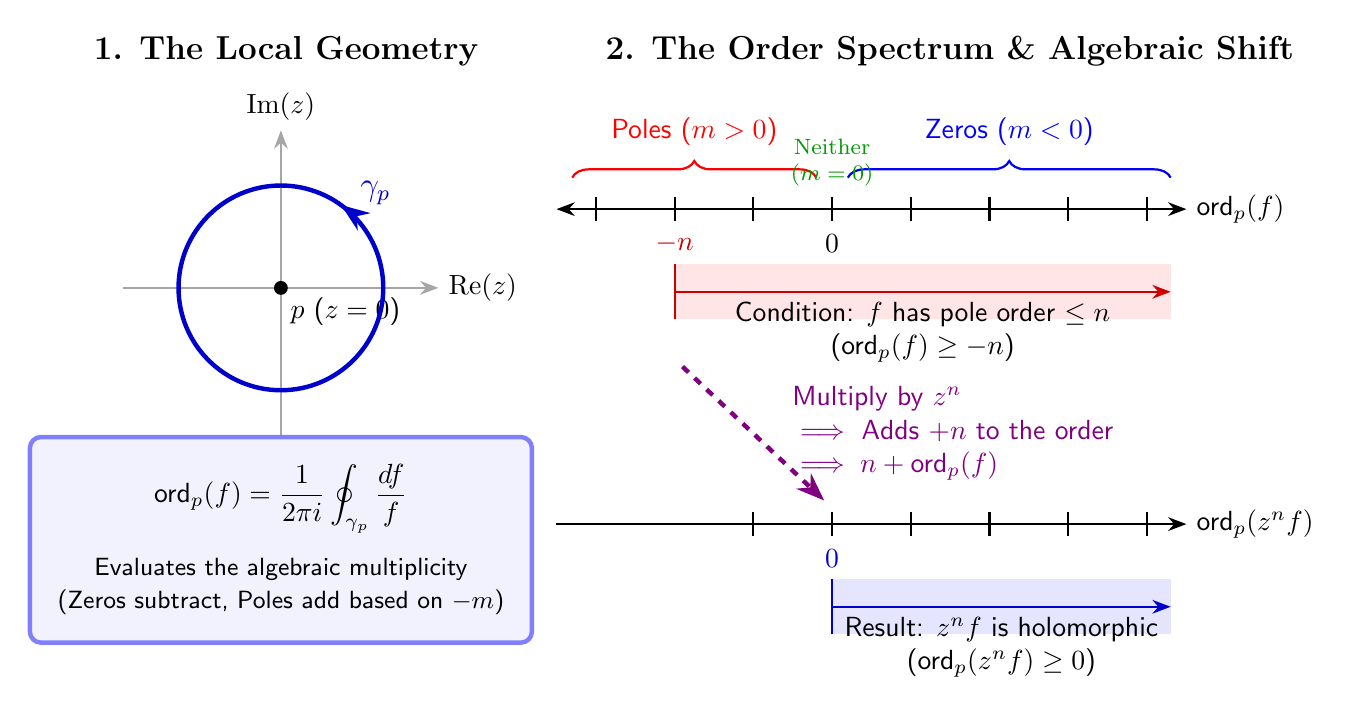
\begin{tikzpicture}[>=Stealth, font=\sffamily]
		
		% =========================================================
		% PANEL 1: Complex Plane and Contour Integral
		% =========================================================
		\begin{scope}[shift={(0,0)}]
			\node[font=\bfseries\large, anchor=west] at (-2.5, 3) {1. The Local Geometry};
			
			% Axes
			\draw[->, gray!70, thick] (-2, 0) -- (2, 0) node[right, text=black] {$\mathrm{Re}(z)$};
			\draw[->, gray!70, thick] (0, -2) -- (0, 2) node[above, text=black] {$\mathrm{Im}(z)$};
			
			% Point p
			\fill[black] (0,0) circle (2.5pt) node[below right] {$p$ ($z=0$)};
			
			% Contour
			\draw[ultra thick, blue!80!black, postaction={decorate, decoration={markings, mark=at position 0.15 with {\arrow{>}}}}] (0,0) circle (1.3);
			\node[blue!80!black, font=\large] at (1.2, 1.2) {$\gamma_p$};
			
			% Definition Box
			\node[draw=blue!50, ultra thick, rounded corners, fill=blue!5, inner sep=10pt, align=center] at (0, -3.2) {
				$\displaystyle \text{ord}_p(f) = \frac{1}{2\pi i}\oint_{\gamma_p}\frac{df}{f}$ \\[8pt]
				\small Evaluates the algebraic multiplicity \\
				\small (Zeros subtract, Poles add based on $-m$)
			};
		\end{scope}
		
		% =========================================================
		% PANEL 2: Order Number Line and the z^n Shift
		% =========================================================
		\begin{scope}[shift={(7, 0)}]
			\node[font=\bfseries\large, anchor=west] at (-3, 3) {2. The Order Spectrum \& Algebraic Shift};
			
			% ----- Top Axis: ord(f) -----
			\draw[<->, thick] (-3.5, 1) -- (4.5, 1) node[right] {$\text{ord}_p(f)$};
			
			% Ticks and nodes
			\foreach \x in {-3,-2,-1,0,1,2,3,4} {
				\draw[thick] (\x, 1.15) -- (\x, 0.85);
			}
			\node[below, font=\bfseries] at (0, 0.8) {$0$};
			\node[below, font=\bfseries, red!80!black] at (-2, 0.8) {$-n$};
			
			% Spectrum Braces
			\draw[decorate, decoration={brace, amplitude=6pt}, thick, red] (-3.3, 1.4) -- (-0.2, 1.4) node[midway, above=8pt] {Poles ($m > 0$)};
			\draw[decorate, decoration={brace, amplitude=6pt}, thick, blue] (0.2, 1.4) -- (4.3, 1.4) node[midway, above=8pt] {Zeros ($m < 0$)};
			\node[align=center, font=\footnotesize, above=2pt, color=green!60!black] at (0, 1.1) {Neither\\($m=0$)};
			
			% Domain: "Pole of order at most n"
			\fill[red!10] (-2, -0.4) rectangle (4.3, 0.3);
			\draw[->, thick, red!80!black] (-2, -0.05) -- (4.3, -0.05) node[midway, below, text=black, align=center] {Condition: $f$ has pole order $\le n$ \\ ($\text{ord}_p(f) \ge -n$)};
			\draw[thick, red!80!black] (-2, -0.4) -- (-2, 0.3);
			
			% ----- The Algebraic Shift -----
			\draw[->, ultra thick, dashed, violet] (-1.9, -1.0) -- (-0.1, -2.7) node[midway, right=10pt, align=left] {Multiply by $z^n$ \\ $\implies$ Adds $+n$ to the order \\ $\implies n + \text{ord}_p(f)$};
			
			% ----- Bottom Axis: ord(z^n f) -----
			\begin{scope}[shift={(0, -4)}]
				\draw[->, thick] (-3.5, 1) -- (4.5, 1) node[right] {$\text{ord}_p(z^nf)$};
				
				\foreach \x in {-1,0,1,2,3,4} {
					\draw[thick] (\x, 1.15) -- (\x, 0.85);
				}
				\node[below, font=\bfseries, blue!80!black] at (0, 0.8) {$0$};
				
				% Domain: "Holomorphic"
				\fill[blue!10] (0, -0.4) rectangle (4.3, 0.3);
				\draw[->, thick, blue!80!black] (0, -0.05) -- (4.3, -0.05) node[midway, below, text=black, align=center] {Result: $z^nf$ is holomorphic \\ ($\text{ord}_p(z^nf) \ge 0$)};
				\draw[thick, blue!80!black] (0, -0.4) -- (0, 0.3);
			\end{scope}
			
		\end{scope}
		
	\end{tikzpicture}
\end{document}